\setlength{\parindent}{4ex}

\chapter{Introduction}
\label{chapter:Introduction} 

This chapter usually includes the following materials: motivation of the problem, existing work, shortcomings of the existing work, the proposed solution, the methodology used to complete the project and implement the solution, outcomes achieved.



\chapter{Related Work}
\label{RelatedWork}

This chapter must include an overview of the current works, their main idea, methodology, outcomes, and shortcomings.
Highlighting shortcomings of existing works is particularly important to motivate the need for the proposed solution.


The following sections present a brief example of a related work section from a paper.


In this chapter, we overview relevant simulation platforms and justify the importance of the FDK.
Also, we summarize existing load balancing and resource allocation schemes and identify their shortcomings when applied to fog-based applications.
Finally, we investigate other existing fog architectures and platforms, and highlight the benefits that the FDK holds over these alternatives.

\section{Simulation Platforms}
\label{SimulationPlatforms}

Due to the significant cost of creating fog and cloud network infrastructures, simulation-based study is the most widely-used approach to evaluate the performance of proposed mechanisms \cite{Skarlat2016resourceprovisioning, ansari2018, yin2018}.

CloudSim \cite{cloudsim} is perhaps the most popular cloud simulation platform available, which is used for modeling the cloud and application provisioning environments. 
It is a discrete event-based simulator written in Java, meaning that it does not actually emulate (virtualize) network entities such as routers and switches.
Instead, CloudSim uses a latency matrix, which contains predefined values for the latency between entities.
Additionally, CloudSim can model dynamic user workloads by exposing a set of methods and variables to configure the resources of simulated VMs.


There are also many extensions to CloudSim, such as CloudSimSDN \cite{cloudsimsdn}, ContainerCloudSim \cite{containercloudsim}, and iFogSim \cite{ifogsim}, which attempt to broaden CloudSim's model to include SDN, container migration simulation, and fog computing, respectively.
However, because CloudSim and these associated extensions are strictly-simulation based, they ultimately do not solve the problems of cost and complexity associated with developing an actual fog application.
Rather, they simply avoid the problem altogether by simulating the entire system. 
Therefore, while CloudSim is a worthy platform for evaluating cloud architectures, load balancing algorithms, etc., it fails to actually serve as a valid fog-based application development platform because projects developed in CloudSim are not portable to a real environment. 
Likewise, the same can be said for most other simulation platforms for similar reasons.

In contrast, the FDK can be used to develop actual fog applications in both physical and emulated environments.
Furthermore, after a fog application is developed in an emulated environment, that application can then be seamlessly ported to a physical environment (and vice versa).


\section{Another subsection}
Continue reviewing the existing works in your area of study.




\chapter{System Architecture}
\label{SystemArchitecture}

The following sections present a brief example of a system architecture section from a paper. Please note how figures, tables, and algorithms are included. 
Also note that figures must be prepared in vector format and included as a PDF file. Do not include JPEG or other image formats.
Use Omnigraffle for Mac Os or Visio for Windows.



Figure \ref{controller} shows the overall fog system architecture including four major components: \textit{controller}, \textit{end-devices}, \textit{switches}, and \textit{fog-devices}.
%
%
%
\begin{figure}[t]
\centering
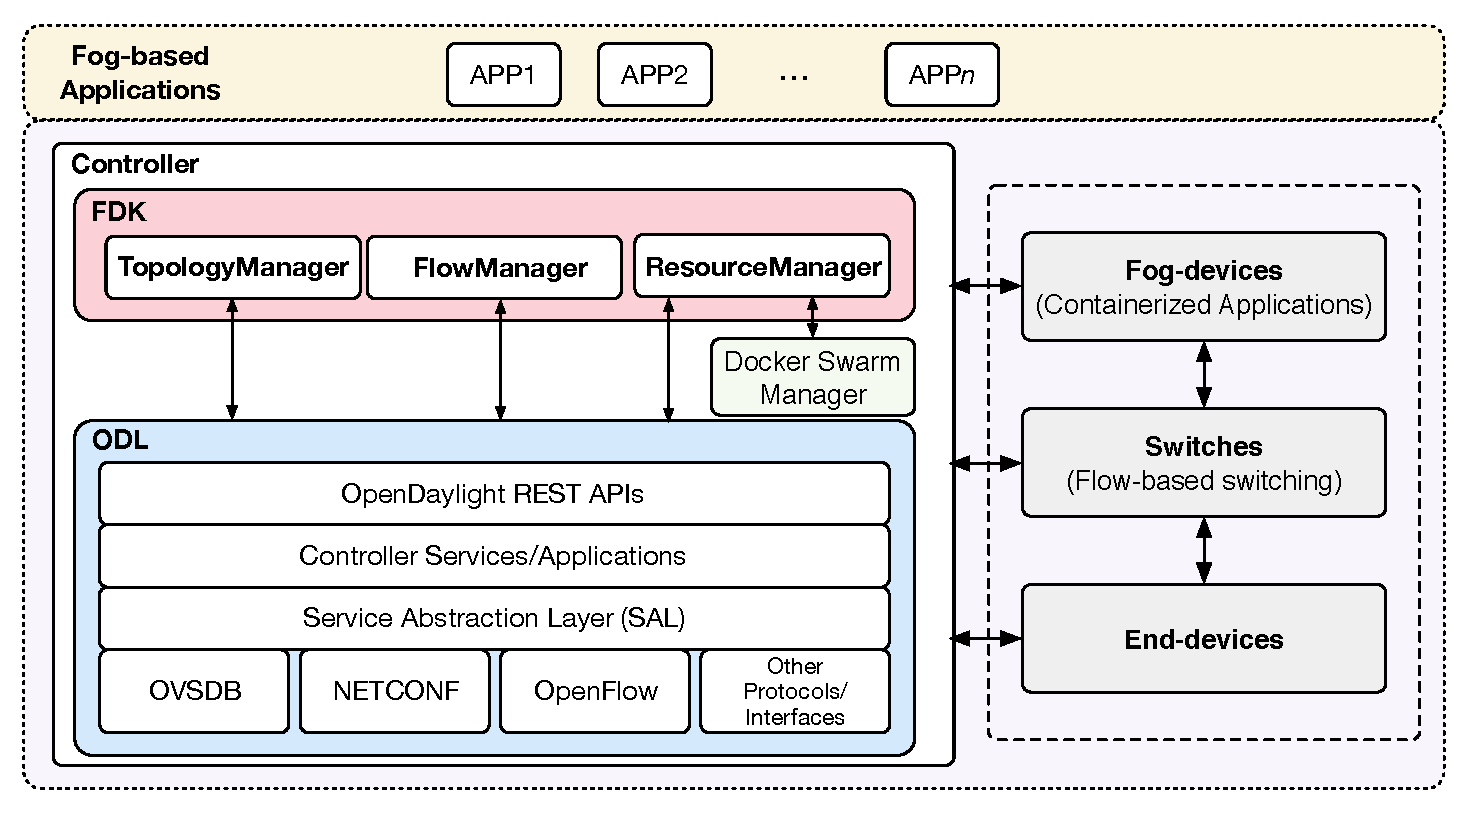
\includegraphics[width=0.8\linewidth]{overall_arch.pdf}
  \captionof{figure}{Overall system architecture.}
  \label{controller}
\end{figure}
%
%
%





\section{FlowManager}
\label{FlowManager}
%
The \textit{FlowManager} component provides a comprehensive interface for the management of OpenFlow flows throughout the network.
The core APIs for this component are described in Table \ref{tab:flowAPIs}.
%
%
\begin{table}[t]
    \centering
    \caption{FlowManager APIs}
    \begin{tabular}{|l|p{7cm}|}
    \hline
    \textbf{API} & \textbf{Description} \\ \hline \hline
    \texttt{\scriptsize{create\_flow()}} & Push OpenFlow flow to switch\\ \hline
    \texttt{\scriptsize{delete\_flow()}} & Delete OpenFlow flow from switch \\ \hline
    \texttt{\scriptsize{track\_flow()}} & Track flow information \\ \hline
    \texttt{\scriptsize{untrack\_flow()}} & Untrack flow information \\ \hline
    \end{tabular}
    \label{tab:flowAPIs}
\end{table}
%
%
First, the FlowManager provides a set of APIs to simplify the process of creating flow table entries on OpenFlow switches.
For example, this component provides a method for creating a \textit{flow skeleton}, which contains all of the basic fields needed to create the flow table entries used by the FDK to enforce traffic paths between end-devices and fog-devices.
Then, the FlowManager's flow-modification APIs can be utilized to further build and shape entries by adding flow actions, flow match fields, and other constructs to a flow skeleton.
For example, flows can be created to match packets by source and destination IP address (or additional identifiers).
Upon a match, multiple actions can be applied to a packet---such as transmitting it through a specific port (used to create network traffic paths) and placing it on a packet queue.
Once a flow table entry is built, the FlowManager's flow-creation APIs can be leveraged to push a newly-built entry to an OpenFlow switch. Similarly, the FlowManager offers flow-deletion APIs that can be used to remove such entries.


\section{ResourceManager}
\label{ResourceManager}
The FDK uses the \textit{ResourceManager} component to manage and allocate all networking and computing resources.
The core APIs of this component are described in Table \ref{tab:resourceAPIs}.
%
%
\begin{table}[t]
    \centering
    \caption{ResourceManager APIs}
    \begin{tabular}{|l|p{8cm}|}
    \hline
    \textbf{API} & \textbf{Description} \\ \hline \hline
    \texttt{\scriptsize{service\_end\_device()}} & Process service requests from end-devices, run the RAA, and instantiate containers \\ \hline
    \texttt{\scriptsize{service\_shutdown\_request()}} & Process shutdown requests, run the RDA, and shutdown containers \\ \hline
    \texttt{\scriptsize{service\_fog\_device()}} & Receive and process resource reporting messages from fog-devices \\ \hline
    \texttt{\scriptsize{resource\_alloc\_algorithm()}} & Attempt to allocate all resources for requested service \\ \hline
    \texttt{\scriptsize{resource\_dealloc\_algorithm()}} & Attempt to deallocate all resources for a service \\ \hline
    \end{tabular}
    \label{tab:resourceAPIs}
\end{table}
%
%
The ResourceManager maintains data structures regarding all resources available in the network.
This is possible with the help of an agent running on every fog-device. 
This agent continually collects and relays information (such as processor and memory utilization) back to the ResourceManager over time.
Similarly, the ResourceManager also repeatedly queries the ODL node inventory to gather current link utilization information.
This information is then stored in the Topology data structure managed by the TopologyManager, which ultimately provides a complete overview of all available resources throughout the network.

The main functionalities provided by the ResourceManager lie within the servers that enable end-devices to request/release computing resources.
These servers act as an interface for managing containerized services and the allocation of resources. % in the fog-devices.
For example, the \textit{service request server} receives and processes requests from end-devices, where each request specifies parameters such as an image name of a containerized service to run and a set of resource requirements for the request.
The image name refers to the type of application processing requested. 
For example, an end-device may specify an image implementing a medical classification application.

Once a request is received, the ResourceManager executes the \textit{resource allocation algorithm} (RAA) presented in Algorithm \ref{RAA}.
If sufficient resources exist, the desired containerized service with the appropriate amount of resources is instantiated on a fog-device, a communication path between the end-device and the fog-device is reserved, and a bandwidth allocation along that path is enforced.
Conversely, the \textit{shutdown request server} provides an interface to revert this process by shutting down containers and deallocating resources.



\SetEndCharOfAlgoLine{}
%%%%%%%%%%%%%%%%%%%%%%%%%%%%%%%%%%%%%%%%%%%%%%%%%%
\begin{algorithm}[!ht]
%\label{RAA}
%SetAlgoLined
%\tiny
\scriptsize
\KwIn{\\
$e_{i} = $ end-device requesting resources\\
$R_{B}(e_{i}) = $ Bandwidth requirement of request from $e_{i}$\\
$R_{P}(e_{i}) = $ Processing requirement of request from $e_{i}$\\
$R_{M}(e_{i}) = $ Memory requirement of request from $e_{i}$\\
Complete topology and resource data (from TopologyManager)\\
}

\BlankLine

\KwOut{\\
A response for $e_{i}$ indicating success or failure\\
}
%
\BlankLine
\BlankLine
$T_{B}(l) = $ Total bandwidth capacity on link $l$ \label{band_all_def_start}\\
$T_{P}(f) =$ Total processing capacity on fog-device $f$\\
$T_{M}(f) =$ Total memory capacity on fog-device $f$\\

\BlankLine
$A_{B}(l) = $ Allocated bandwidth on link $l$\\
$A_{P}(f) =$ Allocated processing on fog-device $f$\\
$A_{M}(f) =$ Allocated memory on fog-device $f$ \label{band_all_def_end} \\

\BlankLine

$\mathcal{N} = $ Set of all nodes \\
$\mathcal{L} = $ Set of all links \\
$\mathcal{F} = $ Set of all fog-devices \\
$\mathcal{F}^{\prime} = \emptyset$ \texttt{//Request servicers} \\
% C is not needed in the algorithm
% We just keep the weight of the link in C, which is already tracked in P!
% $\mathcal{C} = \emptyset$ \texttt{//Lowest-cost dictionary} \\
$\mathcal{P} = \emptyset$ \texttt{//Shortest-path tree} \\
$\mathcal{B} = \emptyset$ \texttt{//Best known link dictionary} \\


\BlankLine
\texttt{//identify request servicers} \\
\For {$f_{j} \in \mathcal{F}$}
{
    \label{raa:createRequestServicers}
    \If {$T_{P}(f_{j}) - A_{P}(f_{j}) > R_{P}(e_{i}) \And$ \\
          $T_{M}(f_{j}) - A_{M}(f_{j}) > R_{M}(e_{i})$} 
    {
        Add $f_{j}$ to $\mathcal{F}^{\prime}$ \\ 
    }
}


%\BlankLine

% No fogs can service the edge request here
\lIf {$\mathcal{F}^{\prime} == \emptyset$}
{
    return FAILURE response \label{raa:failureResponse1}
}

\BlankLine
\label{raa_set_of_nodes}
% $\mathcal{N} = \{e_{i}\}\cup \mathcal{F}^{\prime}\cup \mathcal{S}$\\
%\texttt{{//$\mathcal{H}$ is a min-heap based on path cost from $e_{i}$}} \\
$k = \mathrm{max}(2, \mathrm{size}(\mathcal{L})/\mathrm{size}(\mathcal{N}))$ \\
$\mathcal{H} = minHeap(k)$ \texttt{//K-ary min heap}\\
\BlankLine

% $tmp = (src: e_{i}, dst: e_{i}, src\_port:"", dst\_port:"", weight:0)$ \\
\label{raa:dummy_edge}
$init\_link = (src: e_{i}, dst: e_{i}, weight: 0)$ \\
$\mathcal{H}.\mathrm{push}(init\_link)$ \\
$\mathcal{B}[e_{i}] = init\_link$ \\

\BlankLine
\texttt{//find least-cost paths from $e_{i}$ to fog-devices} \\
\While {$\mathrm{size}(\mathcal{H}) > 0$} 
{
    $u = \mathcal{H}.\mathrm{pop\_min()}$\\
    
    \lIf{$u.src \neq u.dst$} {
        % C is not needed in the algorithm
        % We just keep the weight of the link in C, which is already tracked in P!
        % $\mathcal{C}[u.dst] = u.weight$ \\ 
        $\mathcal{P}[u.dst] = u$ \label{RAAshortestpathadd}
    }
    \BlankLine
    
    \For {$v \in \{ \mathrm{outgoing\;links\;of\;} u.dst\}$}
    {
        \texttt{//v.src is equivalent to u.dst}\\
        %  $cost^{\prime}_{v} = 1/(T_{B}(v) - A_{B}(v) )  $\\
        $v.weight = \mathcal{B}[v.src].weight + 1/(T_{B}(v) - A_{B}(v))$ \label{RAAweight} \\
        \lIf {$(T_{B}(v) - A_{B}(v)) < R_{B}(e_{i})$} {$v.weight = \infty$}
        
        \If{$v.dst \not\in \mathcal{B}$} {
            $\mathcal{H}.\mathrm{push}(v)$ \label{RAApush}\\
            $\mathcal{B}[v.dst] = v$
        }
        \ElseIf{$v.weight < \mathcal{B}[v.dst].weight$} {
            \texttt{//Update link, shift based on weight}\\
            $\mathcal{H}.\mathrm{decrease\_key}(\mathcal{B}[v.dst], v)$ \label{RAAdecreasekey} \\
            $\mathcal{B}[v.dst] = v$
        }
    }
}

\caption{Resource Allocation Algorithm (RAA)}
\label{RAA}
\end{algorithm}








%%%%%%%%%%%%%%%%%%%%%%%%%%%%%%%%%%
%%%%%%%%%%%%%%%%%%%%%%%%%%%%%%%%%%
%%%%%%%%%%%%%%%%%%%%%%%%%%%%%%%%%%

\chapter{Evaluation}
\label{Evaluation}

The following sections present a brief example of a performance evaluation section from a paper. 


In this chapter we first verify the correctness and performance of the FDK using sample applications running on a physical testbed.
We then present simulation-based scalability analysis of the FDK.

\section{Verification and Evaluation using a Physical Testbed} \label{phy_eval}

In this section we verify the correctness and performance of the FDK using a physical testbed running various applications.

\textbf{Testbed.} Figure \ref{physicalInfra} shows our testbed, which includes five OpenFlow switches, four fog-devices, and eight end-devices.
This testbed implements the network presented in Figure \ref{topology}.
Each end-device is a Raspberry Pi Model 3 B+ (running Raspbian Linux) which is connected to a switch using a 1 Gbps cable.
The machine hosting the four fog-devices includes a 4-port Intel 82580 NIC, where each fog-device is a VM associated with a physical port.
Another machine includes five 4-port Intel 82580 NICs as well as a 2-port NIC to build the five OpenFlow switches.
The 2-port NIC is paired with one of the aforementioned 4-port NICs to build a 6-port switch which is connected using a 1 Gbps cable to the controller.
Both machines include two 16-core Intel Xeon CPUs and 64 GB RAM.
Each fog-device and OpenFlow switch uses Ubuntu Server 18.10 and leverages 4 CPU cores and 8 GB of RAM.
The OpenFlow switches run OVS 2.10.0 and support both OpenFlow 1.3 and OVSDB.
Docker daemons run on each fog-device, and are configured to listen for remote TCP connections from the controller.
The controller (including the FDK) is hosted on an external server.
%
%
\begin{figure}[t]
\centering
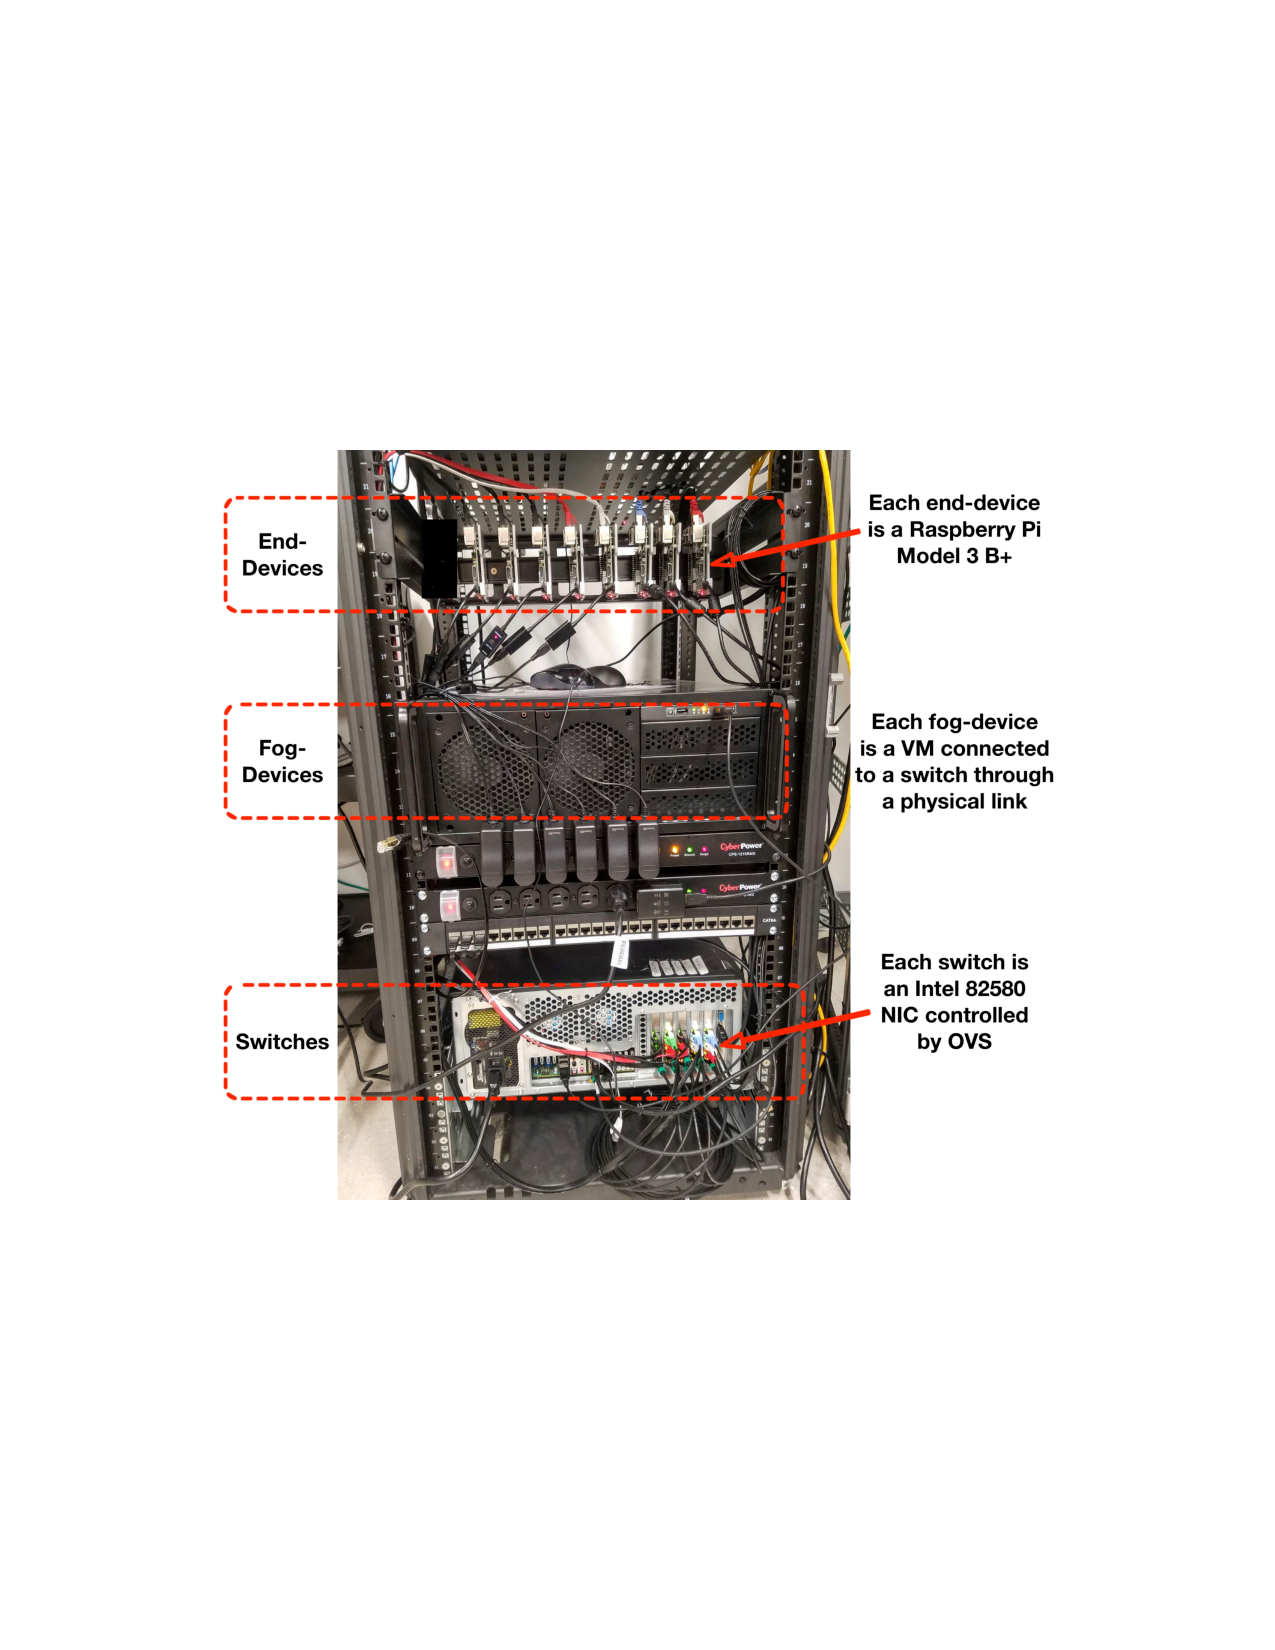
\includegraphics[width=0.75\linewidth]{testbed.pdf}
  \captionof{figure}{The physical testbed used to implement the topology depicted in Figure \ref{topology}.
  End-devices, switches, and fog-devices are connected through physical links.}
  \label{physicalInfra}
\end{figure}



\begin{figure}[t]
\centering
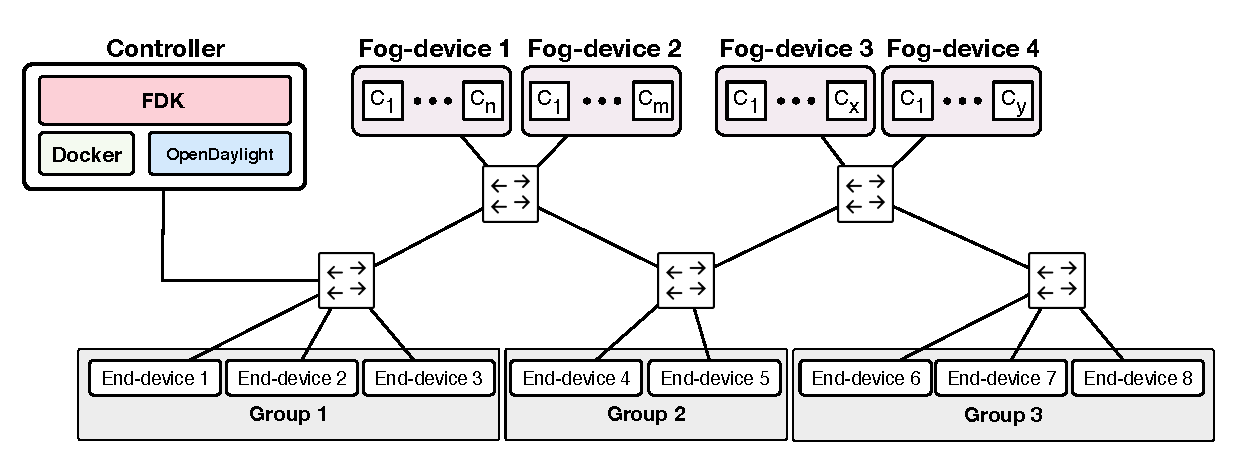
\includegraphics[width=0.95\linewidth]{topology.pdf}
  \captionof{figure}{The network topology used for the development and testing of the FDK. $C_i$ represents a container running on a fog-device.}
  \label{topology}
\end{figure}



\subsection{Test 1: Resource Allocation and Deallocation}
The goal of Test 1 is to characterize the computational and communication overhead of the FDK.
This is accomplished by running applications across all end-devices and recording the runtimes of various operations under different circumstances.
We track the duration of key operations including resource allocation (RAA), resource deallocation (RDA), service request fullfillment, and shutdown request fulfillment.
Service request fulfillment duration refers to the total duration between the time an end-device sends a service request to the FDK and the time the end-device receives a success response from the FDK.
Similarly, shutdown request fulfillment duration refers to the total duration between sending a shutdown request and the reception of confirmation.
For this experiment, we ran \textit{sleep-app} across all eight end-devices in the topology and measured the duration of the aforementioned performance parameters.
We repeated this experiment 250 times for a total of 2000 \textit{sleep-app} runs, and ran two different versions of this test, bringing the number to 4000.
These different test versions are \textit{Test 1a} and \textit{Test 1b}, as follows.


\textbf{Test 1a.} In this test, the end-devices \textit{sequentially} run \textit{sleep-app}.
For example, end-device 1 issues a service request, sleeps for 3 seconds after receiving service, and then issues a shutdown request. 
After completion, the rest of the end-devices perform the same operation sequentially.
Figure \ref{test1a} presents the results of Test 1a.
%
%
\begin{figure*}[t]
\centering
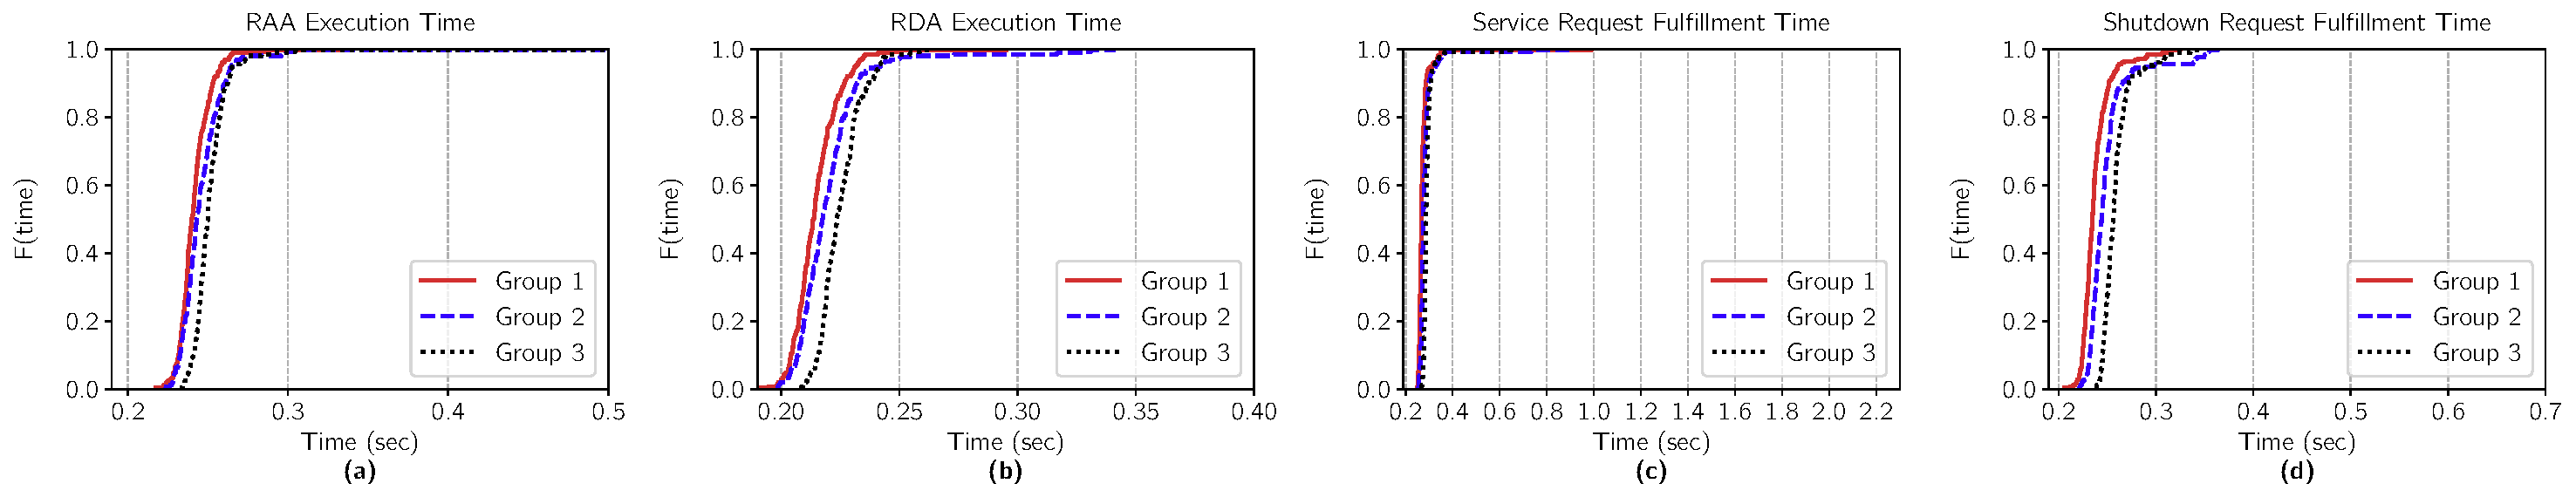
\includegraphics[width=1\linewidth]{test1.pdf}
  \captionof{figure}{Empirical Cumulative Distribution Function (ECDF) graphs for Test 1a. 
  In this test, end-devices issue service requests \textit{sequentially}. 
  Groups closer to the controller (and therefore FDK) complete all of their operations slightly faster than those further from the controller.
  }
  \label{test1a}
\end{figure*}
%
%
The duration of various operations are averaged out among the end-devices of each Group and are then displayed as ECDF graphs.
As seen in Figure \ref{test1a}, more than 95\% of all operations completed within 0.33 seconds across all Groups.
In addition, resource allocation times and service request fulfillment times are nearly identical, as are the resource deallocation times and shutdown request fulfillment times.
This means that resource allocation is the main source of overhead in the process of fulfilling service requests, and that resource deallocation is the main source of overhead in the process of fulfilling shutdown requests.
Also, operations performed for devices in Group 1 tend to finish slightly faster than those for Group 2, which finish faster than those for Group 3.
This is caused by the shorter queuing and packet processing delays along the path to the controller with a fewer number of switches.
However, the difference in timing is on the order of a few milliseconds.






\chapter{Future Work}
\label{FutureWork}


In this chapter we present potential future works to extend the proposed system.




\chapter{Conclusion}
\label{Conclusion}

In this thesis, we proposed...
